\documentclass[10pt,dvipsnames]{beamer}
\usepackage{amsmath,amssymb,longtable,hhline}
\usepackage{mathrsfs}
\usepackage{xcolor}
\usepackage{hyperref}
\usepackage{multicol}
\usepackage{anyfontsize}
\usepackage{minted}
\usepackage{doi}
\renewcommand{\doitext}{DOI:}

\usemintedstyle{tango}
\newcommand{\ltprgsize}{\fontsize{5}{5}\selectfont}
\setminted{fontsize=\ltprgsize,mathescape}

\definecolor{mygreen}{rgb}{0,0.6,0}
\definecolor{mygray}{rgb}{0.5,0.5,0.5}
\definecolor{mymauve}{rgb}{0.58,0,0.82}

\hypersetup{
    bookmarks=true,         % show bookmarks bar?
    unicode=true,           % non-Latin characters in Acrobat’s bookmarks
    pdftoolbar=false,        % show Acrobat’s toolbar?
    pdfmenubar=false,        % show Acrobat’s menu?
    pdffitwindow=false,     % window fit to page when opened
    pdfstartview={FitH},    % fits the width of the page to the window
    pdftitle={Компьютерная алгебра в задачах оптимизации},    % title
    pdfauthor={Evgeny Cherkashin, Seseg Badmatsyrenova},     % author
    pdfsubject={symbolic computations},   % subject of the document
    pdfnewwindow=true,      % links in new PDF window
    colorlinks=true,       % false: boxed links; true: colored links
    linkcolor=red,          % color of internal links (change box color with linkbordercolor)
    citecolor=green,        % color of links to bibliography
    filecolor=magenta,      % color of file links
    urlcolor=blue           % color of external links
}

\usepackage{pifont}

\usetheme{Warsaw}
\usecolortheme{crane}
%\useinnertheme{rectangles}
\setbeamertemplate{itemize item}{\scriptsize\hbox{\donotcoloroutermaths\ding{113}}}
\setbeamertemplate{itemize subitem}{\tiny\raise1.5pt\hbox{\donotcoloroutermaths$\blacktriangleright$}}
\setbeamertemplate{itemize subsubitem}{\tiny\raise1.5pt\hbox{\donotcoloroutermaths$\blacktriangleright$}}
\setbeamertemplate{enumerate item}{\insertenumlabel.}
\setbeamertemplate{enumerate subitem}{\insertenumlabel.\insertsubenumlabel}
\setbeamertemplate{enumerate subsubitem}{\insertenumlabel.\insertsubenumlabel.\insertsubsubenumlabel}
\setbeamertemplate{enumerate mini template}{\insertenumlabel}

\beamertemplatenavigationsymbolsempty

\usepackage{iftex,ifxetex}
\ifPDFTeX
  \usepackage[utf8]{inputenc}
  \usepackage[T1]{fontenc}
  \usepackage[russian]{babel}
  \usepackage{lmodern}
  \usefonttheme{serif}
\else
  \ifluatex
    \usepackage{unicode-math}
    \defaultfontfeatures{Ligatures=TeX,Numbers=OldStyle}
    \setmathfont{Latin Modern Math}
    \setsansfont{Linux Biolinum O}
    \setmonofont{Fira Mono}
    \usefonttheme{professionalfonts}
    % \setmathfont[
    %     Ligatures=TeX,
    %     Scale=MatchLowercase,
    %     math-style=upright,
    %     vargreek-shape=unicode
    %     ]{euler.otf}
  \fi
\fi

%\useoutertheme{split}
%\useinnertheme{rounded}
\setbeamertemplate{background canvas}[vertical shading][bottom=white!80!cyan!20,top=cyan!10]
%\setbeamertemplate{sidebar canvas left}[horizontal shading][left=white!40!black,right=black]

\graphicspath{{pics/}}


% --------------------------

\def\remph#1{\textcolor{Mahogany}{\bfseries #1}}

\begin{document}
\parindent=1em
\title[Supporting IT for Large-scale Resource-driven DES Research]{Information Technologies for Supporting Research of Complex Large-scale Resource-driven Discrete-event Systems Under Uncertainty}
\author[E.~Cherkashin, Q.~Cong, I.~Bychkov, N.~Nagul, A.~Davydov, Y.~Wang, Sh.~Huiyuan]{
\def\and{, }
\remph{Evgeny~Cherkashin}\and
Qiumei~Cong\and
Igor~Bychkov\and
Nadezhda~Nagul\and
Artem~Davydov\and
Yue~Wang\and
Shi~Huiyuan}

\date{${}$\\\vspace{2em}AIIT-2020, October, 16}
\institute{\textit{Matrosov Institute for System Dynamics and Control Theory of SB RAS}, Irkutsk, Russia,
  \href{mailto:eugeneai@icc.ru}{eugeneai@icc.ru}\\
\textit{Liaoning Shihua University, School of Information and Control Engineering,} Fushun, China, \href{mailto:cong_0828@163.com}{cong\_0828@163.com}}
\maketitle
% ----------------------------------------------------------------
\begin{frame}{Large-scale complex Industrial systems}

  With the invention of computers, integrated circuits and communications, information and network communication technology are closely combined with industrial process.

  \remph{Industrial systems} (IS) are union of individual manufacturing and network-computational systems. IS have improved overall operation efficiency and reduced consumption of raw materials.
  \begin{description} \color{MidnightBlue}
  \item[1980-th] better production quality thanks to improved management,
  \item[1990-th] better processes organization (reengineering of business processes),
  \item[2000-th] collaborative manufacturing and management the process between counterparties.
  \end{description}

  Due to the large scale of networked systems, it is difficult to realize the traditional centralized control. The nowadays control structures of large-scale networked industrial processes are \remph{decentralized} and \remph{distributed}.  Decentralized control is simpler in structure and more convenient in implementation, but it does not deal with the physical coupling between subsystems.  Distributed control deals with \remph{coupling relationship} through communication between subsystems, the quality of the communication implies the quality of control.

\end{frame}

\begin{frame}{Batch processing}

  There is three basic models of industrial processes: \alert{continuous}, \alert{discrete}, and \alert{batch processing}.  The most complex one is the third, the batch processing.

  %\begin{examples}
    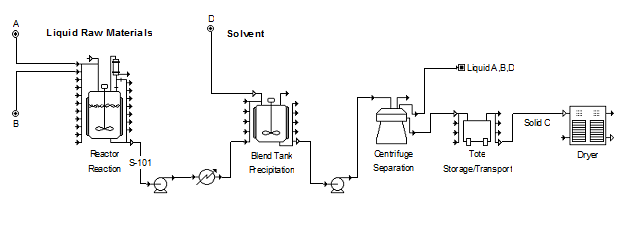
\includegraphics[width=0.9\linewidth]{pics/BatchProcessPFD.png}

  %\end{examples}

\noindent The figures are taken from \url{https://en.wikipedia.org/wiki/Scheduling_(production_processes)}

\end{frame}

\begin{frame}[fragile]{Batch processing}

  \begin{columns}
    \begin{column}{0.5\textwidth}
      \begin{block}{Batch description}
        \tiny
\begin{verbatim}
    Unit Procedure 1: Reaction
        Op 1: Charge A & B (0.5 hours)
        Op 2: Blend / Heat (1 hour)
        Op 3: Hold at 80C for 4 hours
        Op 4: Pump solution through cooler to
              blend tank (0.5 hours)
        Op 5: Clean (1 hour)
    Unit Procedure 2: Blending Precipitation
        Op 1: Receive solution from reactor
        Op 2: Add solvent, D (0.5 hours)
        Op 3: Blend for 2 hours
        Op 4: Pump to centrifuge for 2 hours
        Op 5: Clean up (1 hour)
    Unit Procedure 3: Centrifugation
        Op 1: Centrifuge solution for 2 hours
        Op 2: Clean
    Unit Procedure 4: Tote
        Op 1: Receive material from centrifuge
        Op 2: Load dryer (15 min)
    Unit Procedure 5: Dry
        Op 1: Load
        Op 2: Dry (1 hour)
\end{verbatim}
\end{block}
\end{column}
\begin{column}{0.5\linewidth}
    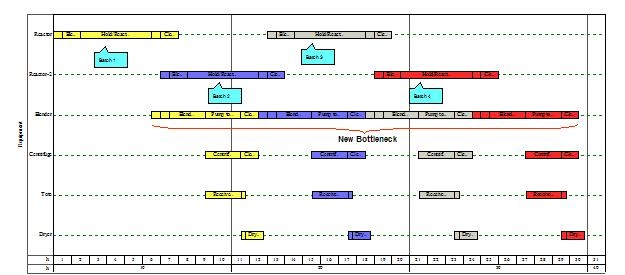
\includegraphics[width=1\linewidth]{pics/BatchCT2.png}
    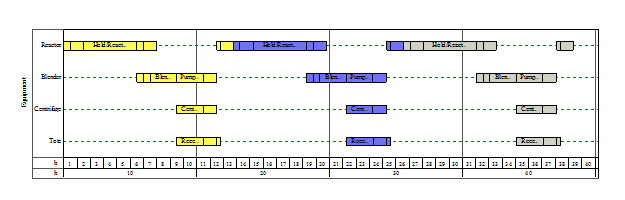
\includegraphics[width=1\linewidth]{pics/BatchCT3.png}
    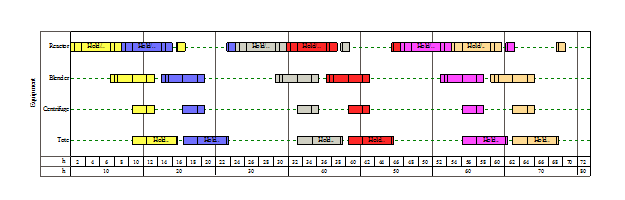
\includegraphics[width=1\linewidth]{pics/BatchCT4.png}
\end{column}
  \end{columns}
\noindent The figures are taken from \url{https://en.wikipedia.org/wiki/Scheduling_(production_processes)}
\end{frame}

\begin{frame}{Batch proceedings visualization}

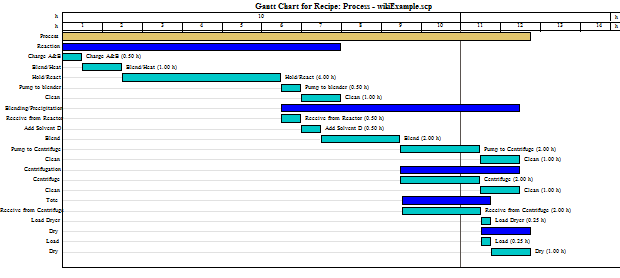
\includegraphics[width=0.7\linewidth]{pics/BatchGantt1.png}

\hfill    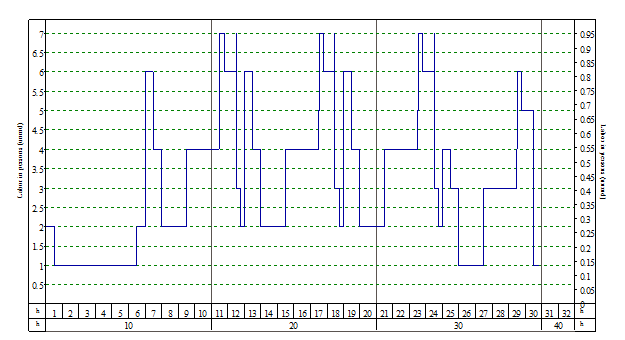
\includegraphics[width=0.7\linewidth]{pics/BatchLabor1.png}

    \noindent The figures are taken from \url{https://en.wikipedia.org/wiki/Scheduling_(production_processes)}
\end{frame}


\begin{frame}{Modeling}
  Representing industrial system as discrete-event system (DES), as some other technical and natural objects, almost always we deal with consumption, production and concurrent temporal acquiring resources.

  Examples of the kind are
  \begin{enumerate}
  \item computer networks;
  \item resource allocation in computer cloud systems;
  \item automated manufacturing; air traffic control;
  \item robotic assembly lines;
  \item highly integrated command, control, communication, and information systems, \emph{e.g.}, groups of underwater autonomous vehicles.
  \end{enumerate}

  \alert{Uncertainties} are classified in \alert{external} and \alert{internal}, \alert{event-based} and \alert{resource-based}.  Uncertainties, as events of DES generated by the environment of the industrial system, can be represented with game theory.  This representation will model the behaviors of external agents (\emph{e.g.} firms, teams, or individuals) under different \alert{competition} and \alert{collaboration} strategies.  Resource-based uncertainties usually represent shortage of resources (utilities).
\end{frame}

\begin{frame}{Example of a Discrete Event System}
\begin{columns}
  \begin{column}{0.5\linewidth}\centering
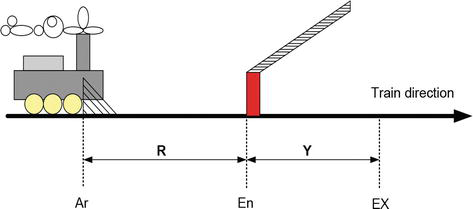
\includegraphics[width=0.8\linewidth]{train.png}
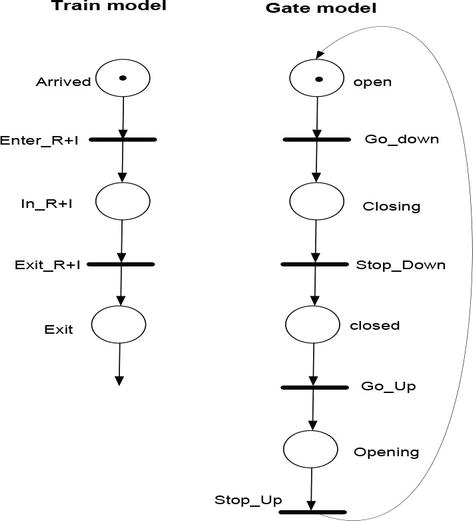
\includegraphics[width=0.8\linewidth]{no-control.png}
\end{column}
\begin{column}{0.5\linewidth}\centering
  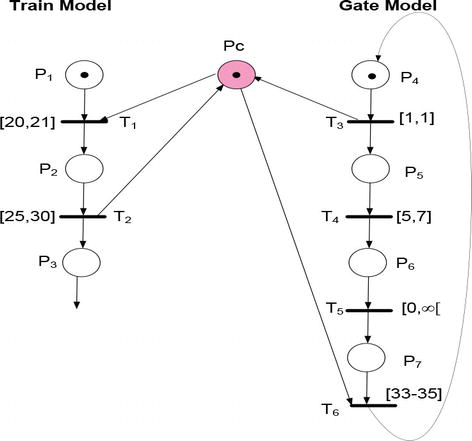
\includegraphics[width=0.8\linewidth]{controlled.png}
  Synthesized supervisory control
\end{column}
\end{columns}
\vfill
\noindent Hamdy Awad, Supervisory Control Systems: Theory and Industrial Applications. 2018. \doi{10.5772/intechopen.75166}
\end{frame}

\begin{frame}{Existing approaches}
  Aim of control is to retain IS near a \textbf{set point} or correspond to a \textbf{set of constraints}.
  \begin{itemize}
  \item Environment generates events, industry reacts. A set of reacting rules must be synthesized.
  \item Mean field games. Number of agents are infinite, continuous mathematic methods are applied.
  \item Predictive control, a model-based optimization. Model predicts the future states with \alert{receding horizon} strategy.
    \begin{itemize}
     \item \alert{distributed cooperative control} of relatively
       independent subsystems, lowering computational complexity.
     \item with limited resources and asynchronous coordination.
     \item with structural uncertainties (equipment failure, illness of staff), resource reserves are accounted.
     \end{itemize}
  \item Fuzzy and neural network methods (blackbox).
  \end{itemize}

  We propose to represent IS with its environment as DES, which behavior described by resource-based games.  In this case we could apply methods of supervisor control synthesis in addition to the predictive techniques.
\end{frame}

\begin{frame}{Predictive control with receding horizon strategy}
  \centering
  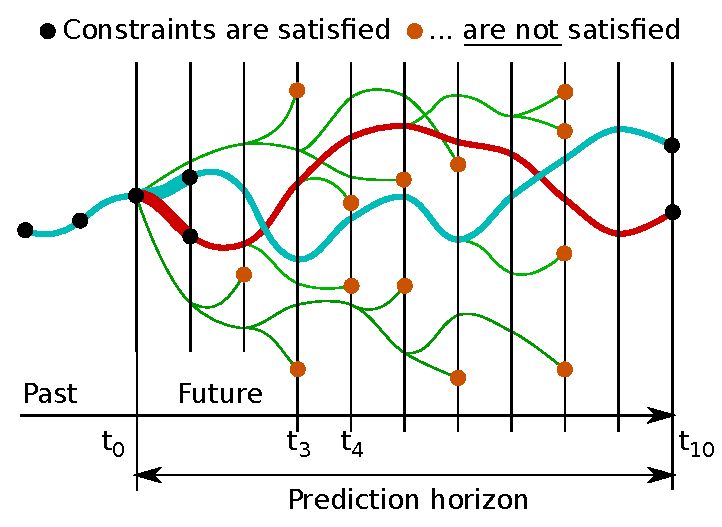
\includegraphics[width=\linewidth]{predictive-horizon.pdf}
\end{frame}

\begin{frame}{Aim of the research}
\textbf{The aim is} the development of new methods of intelligent control synthesis for resource-driven DES with uncertainties is based on
\begin{enumerate}
\item new declarative means in aspects of: event occurrence, state change, resource consumption/production and acquiring, competitor behavior, \emph{etc}.;
\item devising approaches to visual definition of the model with UML, SysML, BPMN, CMMN;
\item development modular supervisors by means of logical inference;
\item adaptation of existing logical inference approaches to support resource-driven games;
\item devising a software for DES description and its computer simulation.
\item represent near-to-real manufacturing processes as RDDESU;
\item testing the methods and software in manufacturing control.
\end{enumerate}

\textbf{Using automation is due to the complexity and scale of the problem.}
\end{frame}

\begin{frame}[fragile]{Resource-based games}
\noindent  $S=\langle v_0,R,F \rangle,$ where $v_0$ is a multiset, $v_0=\{4\cdot(a,A),8 ⋅ (b, A), 9 ⋅ (c, A),$
  $6 ⋅ (a, B), 10 ⋅ (b, B), 3 ⋅ (c, B), 12 ⋅ (d, B), 1 ⋅ A\}$.

  \noindent  Rules, defining agents' behavior:\\
$(r_1^A): \{1 \cdot  A, 2 \cdot  (a, A), 1 \cdot  (b, A)\} → \{−1 \cdot  (a, B), −1 \cdot  (d, B), 1 \cdot  B\},$
$(r_2^A): \{1 \cdot  A, 1 \cdot  (a, A), 3 \cdot  (b, A)\} → \{−2 \cdot  (a, B), 1 \cdot  B\},$
$(r_3^A): \{1 \cdot  A, 1 \cdot  (a, A), 2 \cdot  (b, A), 3 \cdot  (c, A)\} → \{−1 \cdot  (b, B), −4 \cdot  (d, B), 1 \cdot  B\},$
$(r_1^B): \{1 \cdot  B, 3 \cdot  (a, B), 2 \cdot  (b, B)\} → \{−2 \cdot  (a, A), −1 \cdot  (b, A), 1 \cdot  A\},$
$(r_2^B): \{1 \cdot  B, 3 \cdot  (a, B), 2 \cdot  (b, B)\} → \{−4 \cdot  (c, A), 1 \cdot  A\}.$

\noindent Filter conditions:

\begin{columns}
    \begin{column}{0.45\linewidth}
$(C_1^A): (a, A) ≥ 2,$\\
$(C_2^A): (b, A) ≥ 4,$\\
$(C_3^A): (c, A) \to max,$\\
$(C_4^A): (d, B) \to min,$\\
$(C 5A ): (b, B) ≤ 2,$\\
\alert{$F_A = \{C_1^A,\ldots, C_5^A\}$ is A-\bfseries goal}.
    \end{column}
    \begin{column}{0.45\linewidth}
$(C_1^B): (a, B) ≥ 3,$\\
$(C_2^B): (b, B) ≥ 5,$\\
$(C_3^B): (c, A) \to min,$\\
$(C_4^B): (b, A) ≤ 3,$\\
\mbox{$$}\\
\alert{$F_A = \{C_1^B,\ldots, C_4^B\}$ is B-\bfseries goal.}
    \end{column}
  \end{columns}
\vfill
\noindent The example is taken from Igor Sherement's ICCS-DE~2020 paper \url{http://ceur-ws.org/Vol-2638/paper22.pdf}.
\end{frame}

\begin{frame}
  \frametitle{System modeling. SysML }
  \centering
    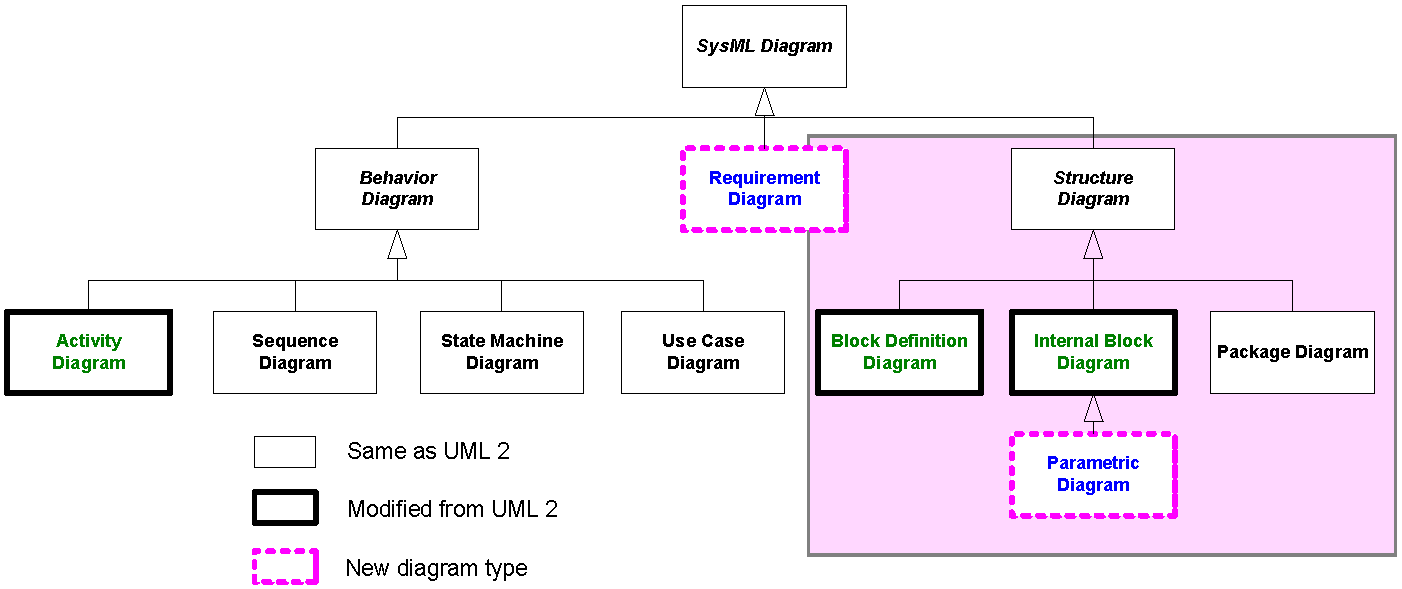
\includegraphics[width=1\linewidth]{qms-pics/diagrams.pdf}
\end{frame}
\begin{frame}
  \frametitle{System modeling. Requirements Diagram}
  \centering
    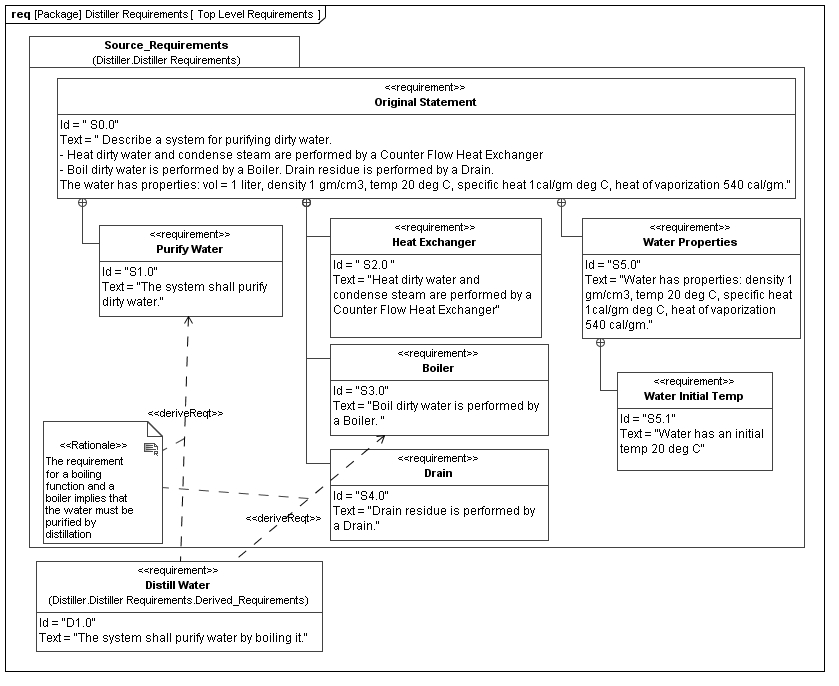
\includegraphics[width=0.9\linewidth]{qms-pics/req-ex.png}
\end{frame}
\begin{frame}
  \frametitle{System modeling. Parametric Diagram}
  \centering
    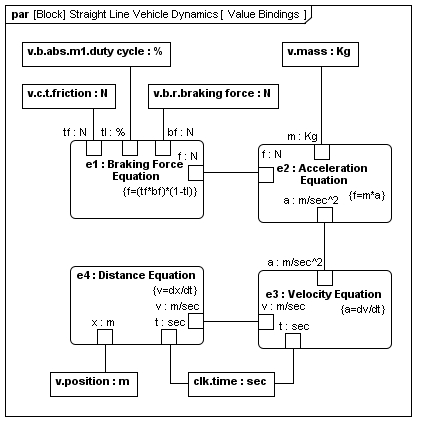
\includegraphics[width=0.7\linewidth]{qms-pics/par-ex.png}
\end{frame}
\begin{frame}
  \frametitle{System modeling. BPMN2.0}
  BPMN -- Business process modeling notation
  \centering
    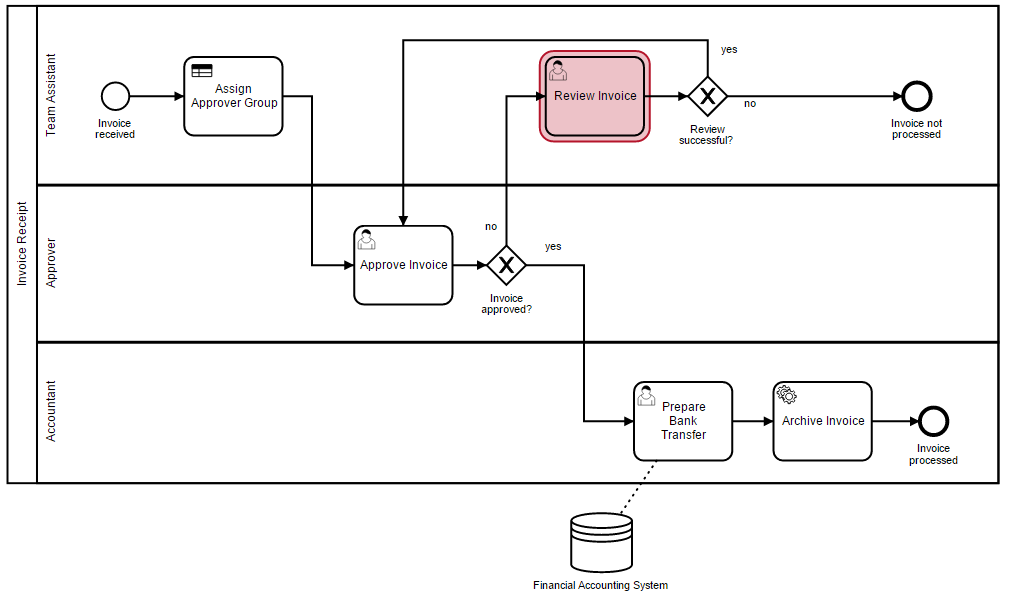
\includegraphics[width=1\linewidth]{qms-pics/bpmn.png}
\end{frame}
\begin{frame}
  \frametitle{System modeling. CMMN1.1}
  CMMN -- Case management model and notation
  \centering
    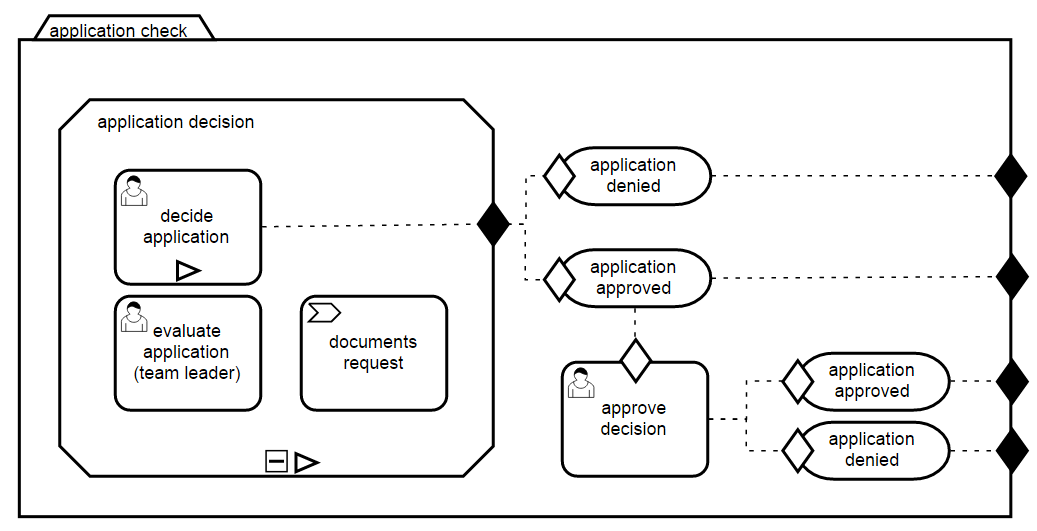
\includegraphics[width=1\linewidth]{qms-pics/cmmn.png}
\end{frame}


\begin{frame}{Control synthesis}
  \begin{enumerate}
  \item DES control is synthesized algorithmically by analysis the controlled automaton. The synthesized control (subautomaton) prevents occurring events shifting system out of admissible state set.
  \item Modifiers of inference rule the default strategy of PCFs were designed for that purpose. The control is synthesized while making proofs.
  \item If the synthesis is not possible, it shows structural elements, preventing the synthesis.
  \item The same was done for language representation of the DSS.
  \item Decentralized control tested on controlling formations of UAVs.
  \end{enumerate}
  Another way is use of forward-chaining inference like receding horizon in RTS mode, where inference stops as soon as time is up.  At each step set of constraint are tested, the admissible states form resulting trajectories and control.
\end{frame}

\begin{frame}{Further activities: Expected results}
\begin{enumerate}
\item A technique for representation complex of models, data structures.
\item Adaptation of standard visual notations (UML, SysML, \ldots).
\item Transformation of the visual models to the internal representation.
\item Methods of synthesizing supervisors for the DES on the base of automatic theorem proving in PCFs.
\item Device new techniques of constructive inferences constructions adopted to the subject of research.
\item Modular automated research software on the base of computer simulation of predictive control with our extensions.
%\item Techniques of the near-to-real manufacturing process formulation as complex of visual models will be developed.
%\item An extensive testing on real industrial processes.
\end{enumerate}
LNHU will perform the following activities:
\begin{enumerate}
\item Research of resource-driven multi-objective optimization: optimal set point and the coordinating multi-objective strategy.
\item Research of distributed predictive control for RDDESU systems with regards of industrial scale and complexity.
\item The establishment of visualization model of ethylene and polypropylene production.
\item Application of the proposed control techniques in petrochemical processes accounting the uncertainties.
\end{enumerate}

\noindent\textbf{The software aimed at CAE/CAM systems development for IS.}
\end{frame}

\begin{frame}{Conclusion}
  The talk was devoted to assess the applicability of existing methods, algorithms and software for construction of \textbf{automated research} software for synthesis of control for three-layer advanced industrial process control models.
  \begin{itemize}
  \item Planning, a composition of the batch processing line.
  \item Scheduling, execution of the plan, utilizing and producing resources.
  \item Control of dynamic of the scheduling with synthesis of DES control supervisors and admissible trajectories in the predictive control mode.
  \end{itemize}

  The enrichment of the convenient standardized two-level model with resource-based game theory enables us to decompose the sources of uncertainties ain a image and likeliness of industry modeling subunits as agents of multi-agent systems.

\end{frame}


\begin{frame}{}
  \vfill
  \centering
  \Huge \textbf{Thank You for attention!}
  \vfill
  
\includegraphics[width=0.5\linewidth]{qr-ind.png}\\
  \normalsize\url{https://github.com/eugeneai/papers-aiit-2020/raw/master/talk-AIIT-2020-10-16-cherkashin-1.pdf}
\end{frame}


\end{document}

%%% Local Variables:
%%% mode: latex
%%% TeX-master: "talk-2020-09-03-proposal.tex"
%%% End:
